\documentclass[12pt, a4paper]{article}
\usepackage[english]{babel}
\usepackage{titlesec}

% \titleformat{\chapter} % command [display] % shape {\bfseries\huge} % format
%   {Chapter \thechapter} % label {0pt} % sep {} % before-code


\usepackage[T5]{fontenc}
\usepackage{mathptmx}[ptm]
\usepackage{a4wide, amssymb, epsfig, latexsym, array, hhline, fancyhdr}
\usepackage[normalem]{ulem}
%\usepackage{soul}
\usepackage{float}
\usepackage[makeroom]{cancel}
\usepackage{amsmath}
\usepackage{amsthm}
\usepackage{multicol, longtable, amscd}
\usepackage{diagbox}%Make diagonal lines in tables
\usepackage{booktabs}
\usepackage{alltt}
\usepackage[framemethod=tikz]{mdframed}% For highlighting paragraph backgrounds
\usepackage{indentfirst}
\usepackage{caption,subcaption}
\usepackage{svg}
\graphicspath{ {figures/} }
\usepackage{lastpage}
\usepackage[lined,boxed,commentsnumbered]{algorithm2e}
\usepackage{enumerate}
\usepackage{color}
\usepackage{graphicx}% Standard graphics package
\graphicspath{ {figures/} }
\usepackage{array}
\usepackage{tabularx, caption}
\usepackage{tabularray}
\usepackage{multirow}
\usepackage{multicol}
\usepackage{rotating}
\usepackage{graphics}
\usepackage{geometry}
\usepackage{setspace}
\usepackage{epsfig}
\usepackage{tikz}
\usepackage[numbers]{natbib}
\usepackage{subcaption}

\usepackage{dirtree}



\usetikzlibrary{arrows, snakes, backgrounds, calc}
\usepackage[unicode]{hyperref}
\hypersetup{urlcolor=blue,linkcolor=black,citecolor=black,colorlinks=true} 

\usepackage{xcolor}

\definecolor{codegreen}{rgb}{0,0.6,0}
\definecolor{codegray}{rgb}{0.5,0.5,0.5}
\definecolor{codepurple}{rgb}{0.58,0,0.82}
\definecolor{backcolour}{rgb}{0.95,0.95,0.92}

\usepackage{listings}
\lstdefinestyle{mystyle}{ backgroundcolor=\color{backcolour},   
    commentstyle=\color{codegreen}, keywordstyle=\color{magenta},
    numberstyle=\tiny\color{codegray}, stringstyle=\color{codepurple},
    basicstyle=\ttfamily\footnotesize, breakatwhitespace=false,         
    breaklines=true,                 
    captionpos=b,                    
    keepspaces=true,                 
    numbers=left,                    
    numbersep=5pt,                  
    showspaces=false,                
    showstringspaces=false, showtabs=false,                  
    tabsize=2 }
\lstset{style=mystyle}



\def\thesislayout{	% A4: 210 × 297
	\geometry{ a4paper, total={160mm,240mm},  % fix over page
		left=30mm, top=30mm, } }
\thesislayout

%\usepackage{fancyhdr}
\setlength{\headheight}{40pt}
\pagestyle{fancy}
\fancyhead{} % clear all header fields
\fancyhead[L]{
 \begin{tabular}{rl}
    \begin{picture}(25,15)(0,0) \put(0,-8){
\includegraphics[width=10mm,
    height=10mm]{Images/hcmut.png}}
    %\put(0,-8){\epsfig{width=10mm,figure=hcmut.eps}}
   \end{picture}&
	%
\includegraphics[width=8mm, height=8mm]{hcmut.png} & %
	\begin{tabular}{l}
        \textbf{ Ho Chi Minh City University of Technology } \\
        \textbf{ Faculty of Computer Science and Engineering }
	\end{tabular} 	
 \end{tabular}
} \fancyhead[R]{
	\begin{tabular}{l}
		\tiny \bf \\
		\tiny \bf \end{tabular}  } \fancyfoot{} % clear all footer fields
\fancyfoot[L]{\scriptsize Big data (CO) - Academic year 2024 - 2025}
\fancyfoot[R]{\scriptsize  Page {\thepage}/\pageref{LastPage}}
\renewcommand{\headrulewidth}{0.3pt}
\renewcommand{\footrulewidth}{0.3pt}

%%%%%%%%%%%%%%%%%%%%%%%%%%%%%%%%%%%%%%%%%%
% Tạo một môi trường mới cho các bảng đặc tả UC, giúp định dạng kiểu
\newenvironment{usecase_table}[1][Test]
{
\begin{table}[H]
% Left-Right Table padding
    \setlength{\tabcolsep}{6pt}
    \renewcommand{\arraystretch}{1.5}
    % \begin{tabularx}{\textwidth}{bs}
    \def\savedcaption{\caption{#1}}%
    \begin{tabular}{|>{\bfseries} p{0.2\linewidth}|p{0.7\linewidth}|}

} {
    \end{tabular}
    \savedcaption
\end{table}
}

\newenvironment{usecase_enum}
{
    \begin{enumerate*}[itemjoin={\newline}]
} {
    \end{enumerate*}
}

\makeatletter
\newenvironment{acknowledgments}{
	\small
	\begin{center}
	  {\bfseries Acknowledgments\vspace{-.5em}\vspace{\z@}}
	\end{center}
	\quotation
  }{}
\makeatother

% Declaration
\makeatletter
\newenvironment{declaration}{
	\small
	\begin{center}
	  {\bfseries Declaration\vspace{-.5em}\vspace{\z@}}
	\end{center}
	\quotation
  }{}
\makeatother

\makeatletter
\newenvironment{abstr}{
        \small
        \begin{center}
	{\bfseries Abstract \vspace{-.5em}\vspace{\z@}}
        \end{center}
        \quotation
    }{}
\makeatother

\makeatletter
\newenvironment{abstrsss}{
        \small
        \begin{center}
	{\bfseries Abstractss \vspace{-.5em}\vspace{\z@}}
        \end{center}
        \quotation
    }{}
\makeatother
%%%%%%%%%%%%%%%%%%%%%%%%%%%%%%%%%%%%%%%%%%%%%%5
\setcounter{secnumdepth}{4}
\setcounter{tocdepth}{3}
\makeatletter
\newcounter {subsubsubsection}[subsubsection]
\renewcommand\thesubsubsubsection{\thesubsubsection .\@alph\c@subsubsubsection}
\newcommand\subsubsubsection{\@startsection{subsubsubsection}{4}{\z@}%
                                     {-3.25ex\@plus -1ex \@minus -.2ex}%
                                     {1.5ex \@plus .2ex}%
                                     {\normalfont\normalsize\bfseries}}
\newcommand*\l@subsubsubsection{\@dottedtocline{3}{10.0em}{4.1em}}
\newcommand*{\subsubsubsectionmark}[1]{}
\makeatother



\everymath{\color{black}}%make in-line maths symbols blue to read/check easily

\sloppy
\captionsetup[figure]{labelfont={small,bf},textfont={small,it},belowskip=-1pt,aboveskip=-9pt}
%space removed between caption, figure, and text
\captionsetup[table]{labelfont={small,bf},textfont={small,it},belowskip=-1pt,aboveskip=7pt}
\setlength{\floatsep}{5pt plus 2pt minus 2pt}
\setlength{\textfloatsep}{5pt plus 2pt minus 2pt}
\setlength{\intextsep}{10pt plus 2pt minus 2pt}


% Declare a variable named Proc using \newcommand

\newcommand{\Uni}{Ho Chi Minh University - Vietnam National Unversity, Ho Chi Minh City}

\renewcommand{\labelitemi}{\normalfont\bfseries\textendash}
\renewcommand{\labelitemii}{\textbullet}
\renewcommand*\baselinestretch{1.5}\selectfont


\thesislayout

\begin{document}

\begin{titlepage}
    
\begin{tikzpicture}[remember picture, overlay]
        \draw[line width = 4pt] ($(current page.north west) + (1.0in,-0.5in)$)
        rectangle ($(current page.south east) + (-0.4in,0.5in)$);
        \draw[line width=1.5pt]
        ($ (current page.north west) + (1.05in,-0.55in) $) rectangle ($ (current
        page.south east) + (-0.45in,0.55in) $);
    \end{tikzpicture}

    \begin{center}
        \large \textbf{VIETNAM NATIONAL UNIVERSITY, HO CHI MINH CITY} \\
        \large \textbf{HO CHI MINH UNIVERSITY OF TECHNOLOGY} \\
        \large \textbf{FACULTY OF COMPUTER SCIENCE AND ENGINEERING}
    \end{center}

    \begin{figure}[h!]
        \begin{center}
            
\includegraphics[width=5cm]{Images/hcmut.png}
        \end{center}
    \end{figure}

    \begin{center}
        \begin{tabular}{c}
        \multicolumn{1}{l}{\textbf{{\Large Big Data (CO1007)}}}\\
        ~~\\
        \hline
        \\
        \multicolumn{1}{l}{\textbf{{\Large Assignment Report}}}\\
        \\
        \textbf{{\Huge Applying Streaming SQL in}}\\
        \textbf{{\Huge Real-Time Social Media}}\\
        \textbf{{\Huge Interaction Tracking}}\\
        \\
        \hline
        \end{tabular}
        \end{center}

    \vspace{1cm}
    \begin{table}[H]
        \begin{tabular}{rrl}
        \hspace{5 cm} & \textbf{Mentor}: & Thoại Nam \\
        
        & \textbf{Student}: & Trần Hà Tuấn Kiệt -- 2011493 \\
        & & Nguyễn Đức Thuỵ -- 2012158 \\
        \end{tabular}
        \end{table}
    \vspace{1cm}

    \begin{center}
        {\large Ho Chi Minh City, \the\month/\the\year}
    \end{center}
\end{titlepage}


\newpage

%\thispagestyle{empty} \chapter*{Work Assignment} \begin{table}[H] \centering
% \renewcommand{\arraystretch}{1.5} \begin{tabular}{|c|c|c|l|} \hline
% \textbf{No.}       & \textbf{Full name}                 & \textbf{Student ID}
% & \textbf{Work Assignment}                     \\
%         \hline %%%%%Student 1%%%%%%%%%%% \multirow{4}{*}{1} &
%         \multirow{4}{*}{Trần Hà Tuấn Kiệt} & \multirow{4}{*}{2011493} & -
%         Exploratory Data Analysis                  \\
%                            &                                    &
%                            & - System proposal and architecture           \\
%                            &                                    &
%                            & - Research and Develop with new technologies \\
%                            &                                    &
%                            & - Implement system endpoints                 \\
%         \hline %%%%%Student 2%%%%%%%%%%% \multirow{4}{*}{2} &
%         \multirow{4}{*}{Nguyễn Đức Thuỵ}   & \multirow{4}{*}{2012158} & -
%         Exploratory Data Analysis                  \\
%                            &                                    &
%                            & - System proposal and architecture           \\
%                            &                                    &
%                            & - Research and Develop with new technologies \\
%                            &                                    &
%                            & - Implement data processing flows            \\
%         \hline \end{tabular} \end{table} \newpage

% Revert title name back to English
\renewcommand{\contentsname}{Table of Contents}
\renewcommand{\listfigurename}{List of Figures}
\renewcommand{\listtablename}{List of Tables}
\renewcommand{\bibname}{References}
\renewcommand{\figurename}{Figure}

\tableofcontents
\newpage

%\thispagestyle{empty}
\listoffigures
\listoftables
\newpage

% \renewcommand\thechapter{Chapter \arabic{chapter}}

\section{Introduction about Social media Interaction}
\textbf{Social Media Interaction} refers to the ways users engage and
communicate with content, brands, and other users on social media platforms. It
encompasses all forms of engagement, such as likes, comments, shares, mentions,
direct messages, and reactions to posts. These interactions create a dynamic,
two-way communication channel between individuals, communities, and businesses.

Social media interaction encompasses various elements that enable engagement and
communication among users, brands, and communities. Engagement types like likes,
comments, shares, retweets, and mentions, which allow users to express opinions
and amplify content. Direct communication, such as private messages and replies,
facilitates personal connections, while user-generated content (UGC) like
reviews and testimonials highlights the creative involvement of users.
Additionally, community engagement through group discussions and forums fosters
a sense of belonging and collaboration. 

The importance of social media interaction lies in its ability to provide
real-time feedback, offering valuable insights into audience opinions,
preferences, and sentiments. It enhances brand awareness by increasing
visibility and trust, while also allowing businesses to analyze content
performance and measure campaign success. Social media interaction builds strong
relationships between brands and their audiences, encourages loyalty, and helps
identify emerging trends and consumer behaviors. Ultimately, it serves as a
powerful tool for driving meaningful connections and strategic growth in the
digital landscape.

This concept underscores the importance of leveraging unbounded data streams to
stay competitive in the dynamic world of digital engagement. The accompanying
vibrant image of individuals in creative poses reflects the dynamic and lively
nature of social media platforms, aligning with the essence of constant
interaction and engagement.

Let's take a look at a comparison between bounded dataset and unbounded dataset
in data processing.

\begin{figure}[H]
    \centering
    \includegraphics[width=\textwidth]{Images/unbounded-data.png}
    \vspace{1em}
    \caption{Comparison between bounded dataset and unbounded dataset}
    \label{fig:comparison}
\end{figure}

\textbf{A table represents a bounded dataset}, meaning it contains a finite and
complete set of data at any given time. This bounded nature allows for aggregate
or summary calculations, such as counting records or calculating averages. For
example, the query \textbf{`SELECT count(*) FROM orders WHERE price > 100`} can
aggregate the results in the table to produce a deterministic count because the
data is static and complete.

On the other hand, \textbf{streams represent unbounded dataset}, where data
continuously flows in over time. Since streams are ongoing, queries on streams
never actually end; they continuously process incoming data. For example, when
applying the same query to a stream, each incoming event is processed
individually, providing incremental updates to the results. This behavior is
suitable for scenarios such as real-time analytics or monitoring, where data is
continuously generated and processed.

In short, the \textbf{Figure \ref{fig:comparison}} demonstrates this distinction
effectively, showing how tables aggregate finite data into a static result,
while streams generate dynamic, continuously updated outputs. This concept is
essential in understanding how modern data systems like databases, stream
processors, and big data frameworks handle and process information.

\section{Problem Statement}
    \subsection{Impact}
    \textbf{The lack of real-time insights from unbounded social data}
    significantly hampers the ability of businesses and organizations to respond
    promptly to trends and audience engagement. In the fast-paced digital
    landscape, trends evolve rapidly, and audience preferences shift
    dynamically. Without continuous access to real-time data streams, it becomes
    difficult to monitor and analyze social interactions effectively. This delay
    in gaining actionable insights prevents organizations from adapting
    strategies, capitalizing on emerging opportunities, or addressing potential
    challenges in a timely manner. Ultimately, the inability to respond to
    real-time engagement can lead to missed opportunities, reduced
    competitiveness, and weakened connections with audiences, making it crucial
    to leverage tools that process unbounded data streams for effective
    decision-making and sustained growth.
    \subsection{Objectives}
    The objective is to \textbf{implement a real-time social media interaction
    tracking system for platforms} like Mastodon and X (formerly Twitter). This
    system will process and analyze unbounded streams of social media data,
    enabling organizations to monitor user interactions, engagement trends, and
    audience behaviors as they happen. By providing actionable insights in real
    time, it empowers businesses to stay responsive to emerging trends, adapt
    strategies effectively, and maintain relevance in the fast-paced digital
    landscape. This highlights the importance of leveraging advanced data
    processing technologies to manage the dynamic nature of social media,
    ensuring informed and timely decision-making.

    \subsection{Approach}
        \subsubsection{Data Collection}
            \subsubsubsection*{Mastodon}
            Mastodon is a decentralized social media platform structured as a
            \textbf{network of independent servers}, commonly referred to as
            instances. Each instance operates independently, serving unique
            communities and interests, yet they remain interconnected through a
            federated network. This decentralized approach contrasts with
            centralized platforms, fostering diversity and community-specific
            experiences.
            \begin{itemize}
                \item \textbf{Structure:} Mastodon’s ecosystem consists of
                multiple independent servers, each catering to distinct
                communities while participating in a larger, interconnected
                federation.
                \item \textbf{Data access:} Mastodon provides real-time data
                streams through its Server-Sent Events (SSE) API, enabling
                access to ongoing activities like posts, mentions, hashtags, and
                interactions.
                \item \textbf{Data types:} The platform generates various types
                of data, including posts, mentions, hashtags, and user
                interactions, making it a rich source for social media analytics
                and engagement monitoring.
            \end{itemize}
            $\quad$ Mastodon presents unique challenges due to its decentralized
            structure, where data is distributed across numerous independent
            servers (instances). Aggregating and analyzing data from the entire
            network is inherently complex and resource-intensive, requiring
            sophisticated solutions to handle the fragmented ecosystem.
            Additionally, Mastodon's strong emphasis on user privacy, with
            strict controls and regulations, further complicates data collection
            and processing while ensuring compliance with user preferences and
            privacy standards.
            \subsubsubsection*{X (formerly Twitter)}
            X, formerly known as Twitter, operates as a centralized social media
            platform with a unified database, making it distinct from
            decentralized systems like Mastodon. This centralized structure
            provides a single, cohesive source of data, which simplifies access
            and analysis for users, developers, and organizations.
            \begin{itemize}
                \item \textbf{Structure:} X is built on a centralized database
                architecture, enabling streamlined data management and easier
                access to platform-wide information.
                \item \textbf{Data access:} The platform offers real-time
                streams through the X API, allowing developers to track
                activities such as tweets, retweets, likes, mentions, and
                trending topics in real time.
                \item \textbf{Data types:} X generates various types of valuable
                data, including tweets, retweets, likes, mentions, and trends,
                making it a vital source for social media analytics and
                insights.
            \end{itemize}
            $\quad$ X faces notable challenges in its data access and usage policies.
            Strict \textbf{rate limits on API usage} restrict the volume of data that
            can be collected within a specific timeframe, creating barriers to
            conducting comprehensive and large-scale analyses. Additionally,
            \textbf{privacy regulations and API restrictions} further complicate data
            collection and processing, as developers and researchers must
            navigate limitations designed to protect user data while ensuring
            compliance with legal and ethical standards. These challenges
            necessitate innovative solutions to effectively leverage the
            platform's data while respecting its constraints.
            \subsubsection{Concept}
            \textbf{Streaming SQL} is an extension of traditional SQL, specifically designed to handle unbounded, real-time data streams. Unlike standard SQL, which processes finite datasets stored in static tables, Streaming SQL operates on continuous data streams that are constantly being updated, enabling real-time analysis and processing.
            \begin{figure}[H]
                \centering
                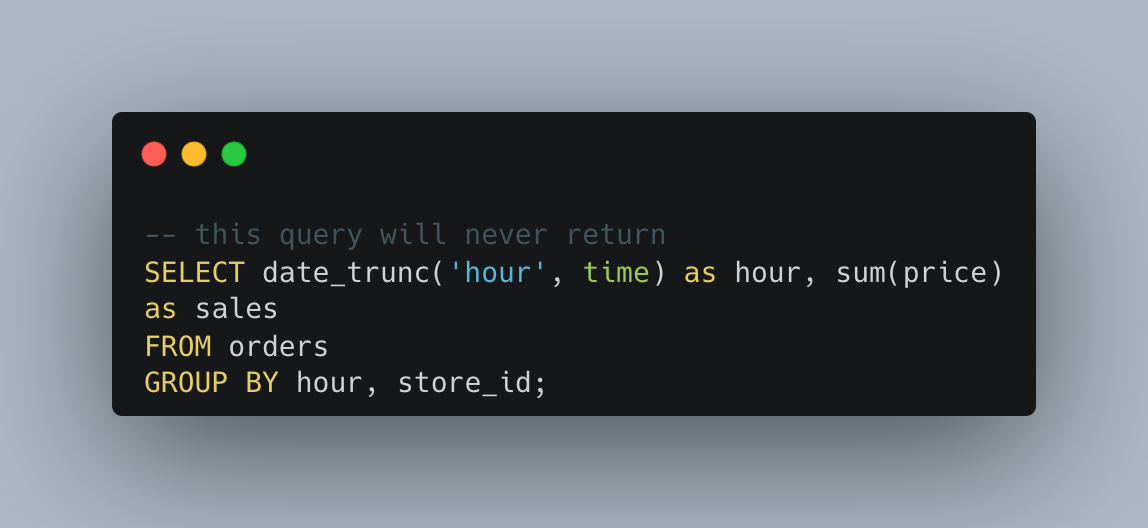
\includegraphics[width=0.7\textwidth]{Images/image (1).png}
                \vspace{1em}
                \caption{Concept of Streaming SQL}
            \end{figure}
            \begin{figure}[H]
                \centering
                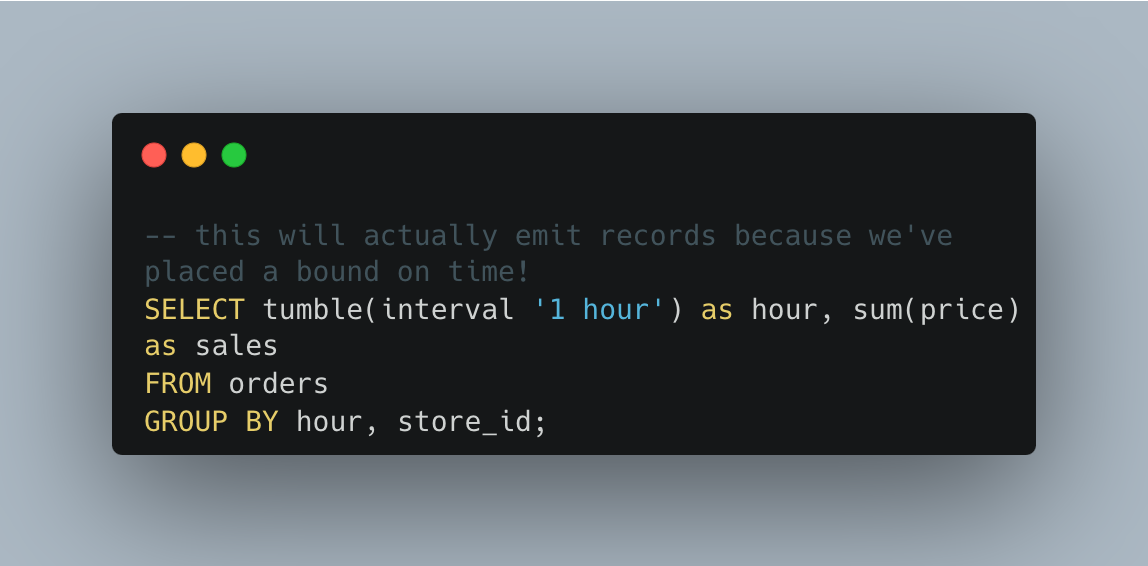
\includegraphics[width=0.7\textwidth]{Images/image (2).png}
                \vspace{1em}
                \caption{Concept of Streaming SQL}
            \end{figure}
            \subsubsubsection*{Dataflow Semantics}
            \begin{figure}[H]
                \centering
                
\includegraphics[width=0.7\textwidth]{Images/row-by-row.png}
                \vspace{1em}
                \caption{Row-by-Row Processing}
            \end{figure}
            \begin{figure}[H]
                \centering
                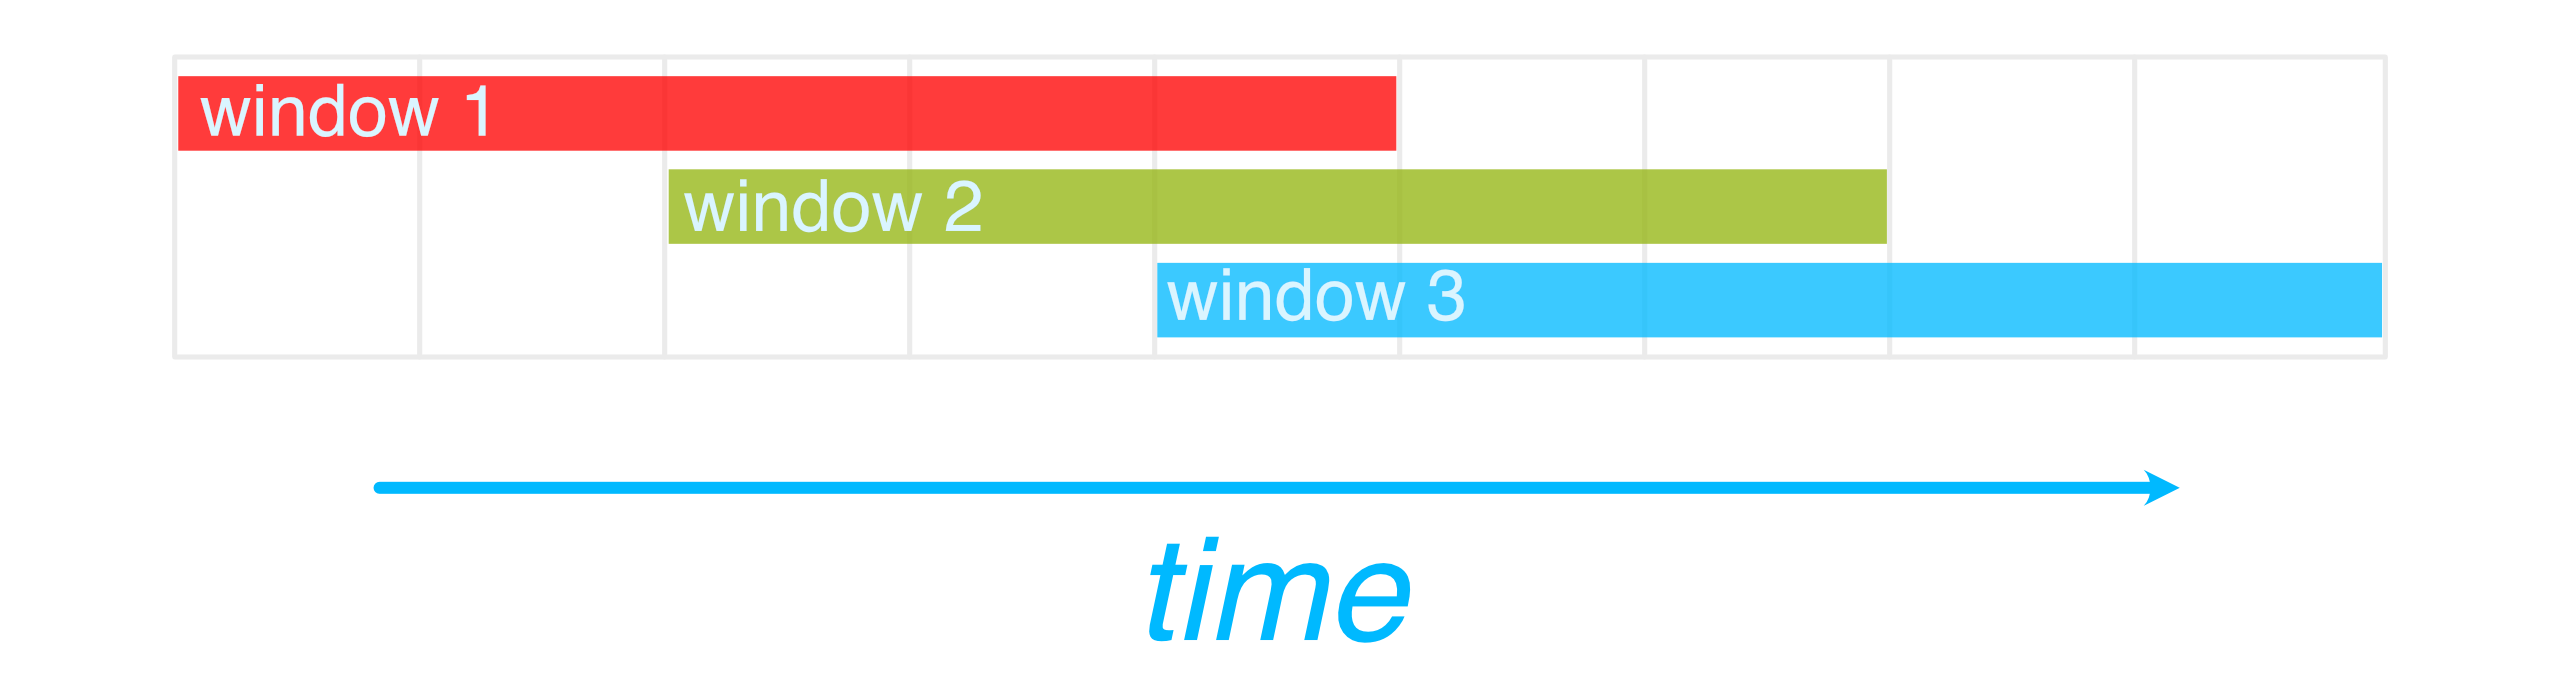
\includegraphics[width=0.7\textwidth]{Images/sliding-window.png}
                \vspace{1em}
                \caption{Sliding windows}
            \end{figure}
            \begin{figure}[H]
                \centering
                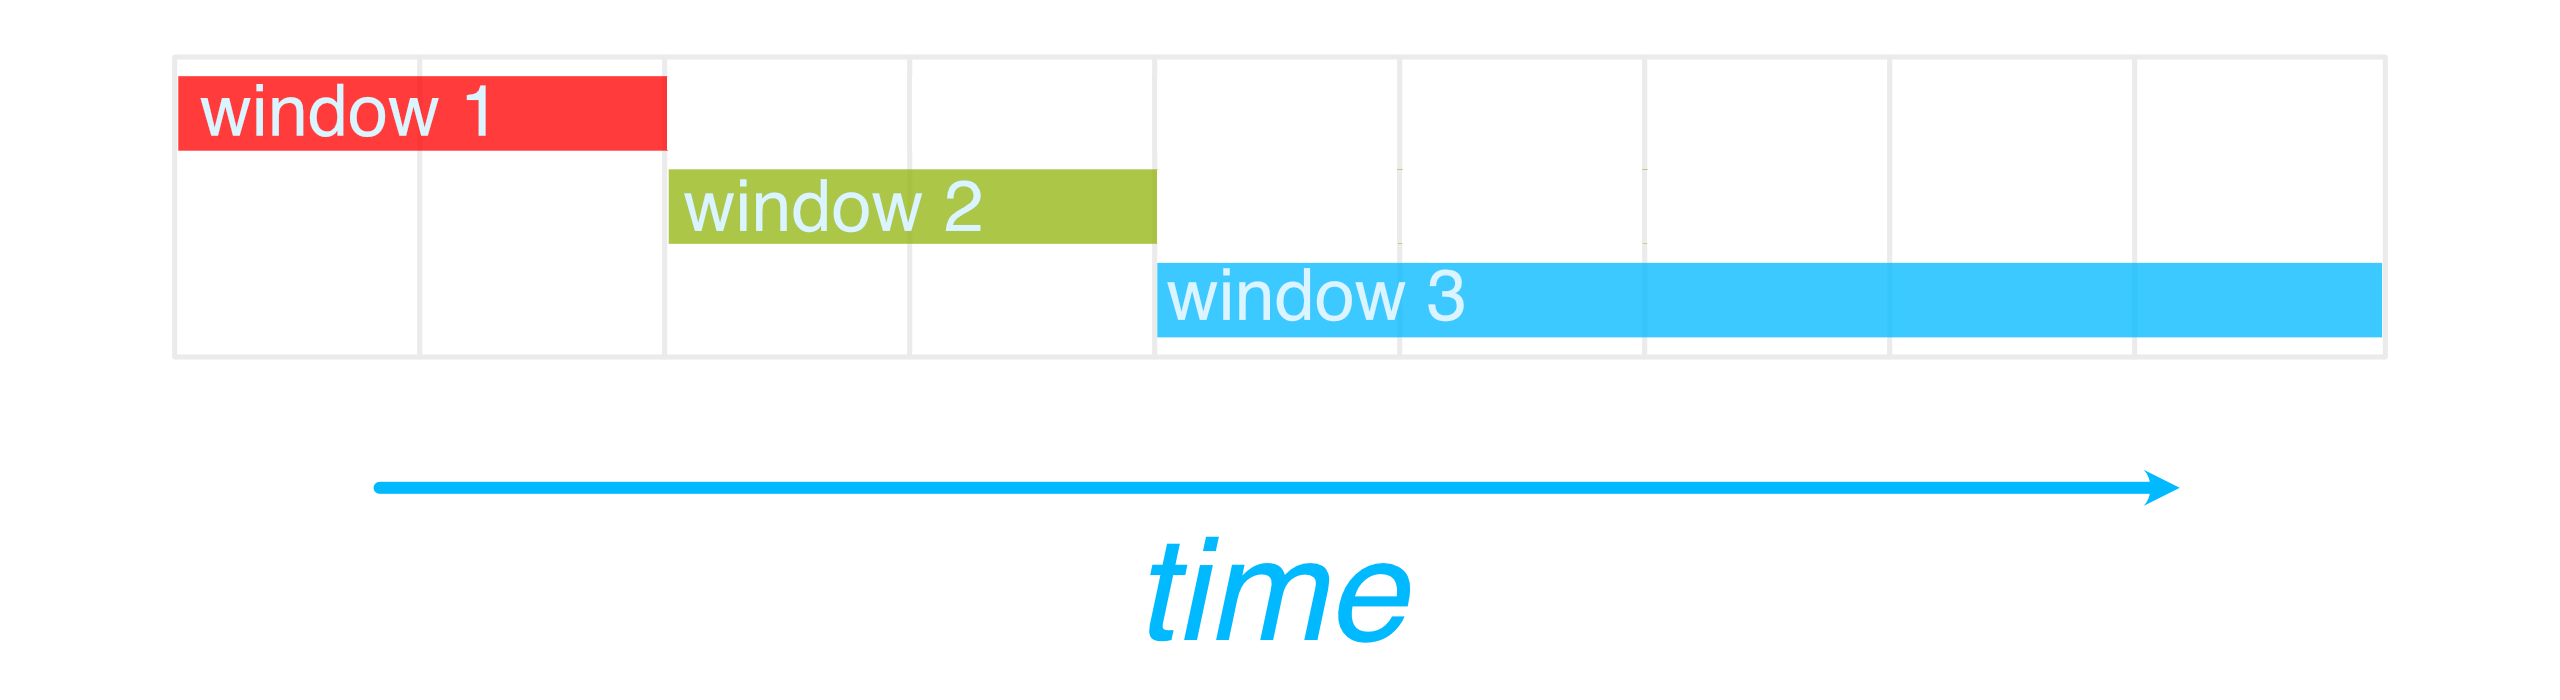
\includegraphics[width=0.7\textwidth]{Images/tumbling-window.png}
                \vspace{1em}
                \caption{Tumbling windows}
            \end{figure}
            \begin{figure}[H]
                \centering
                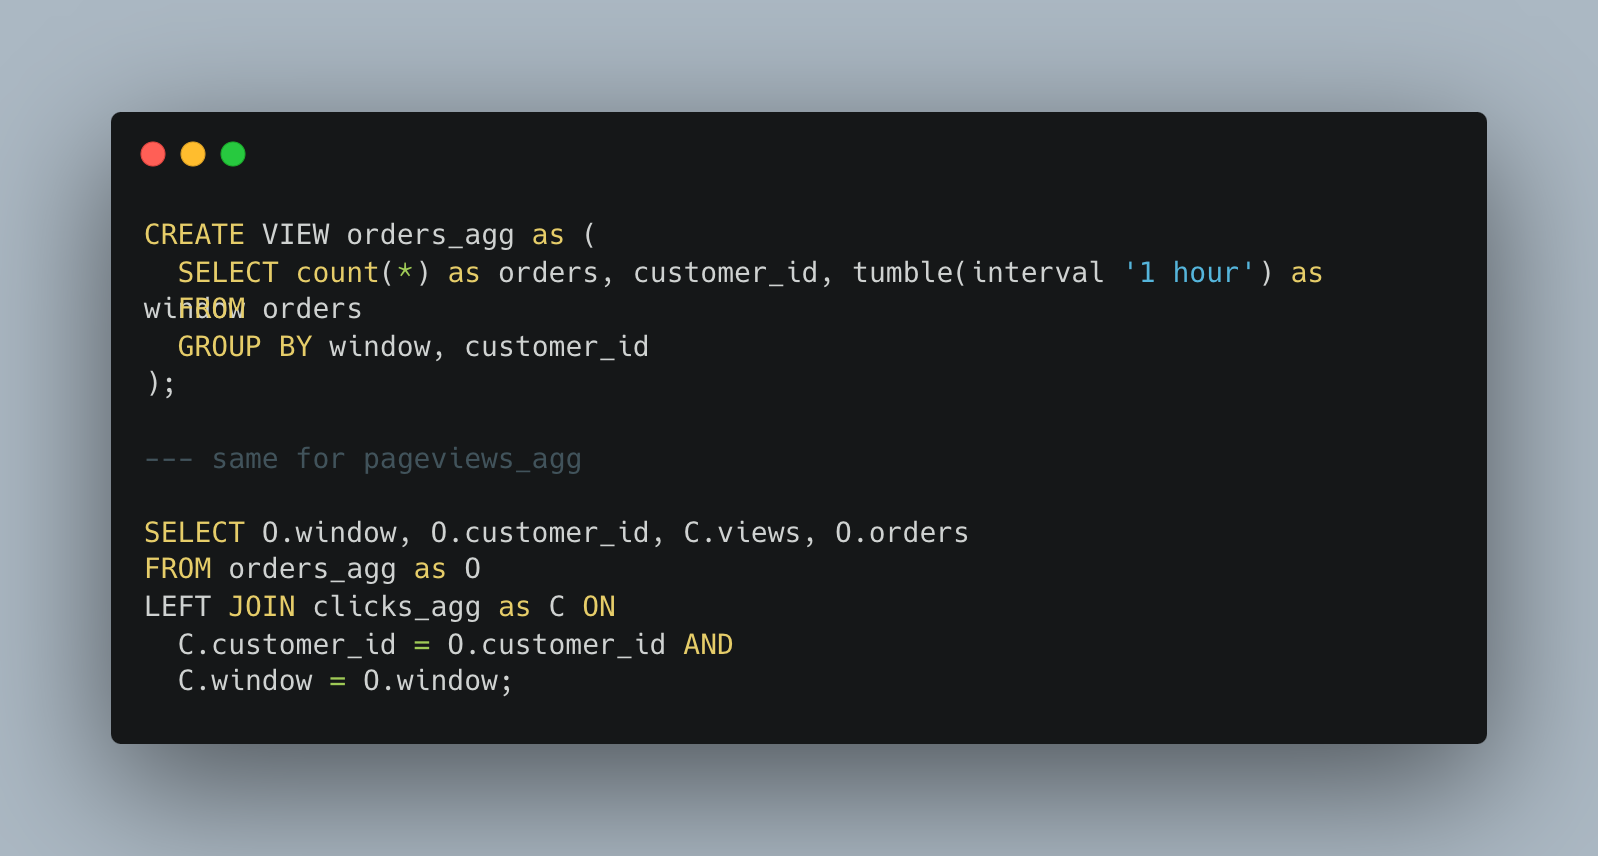
\includegraphics[width=0.7\textwidth]{Images/apply-JOIN.png}
                \vspace{1em}
                \caption{Apply to Join Operation}
            \end{figure}
            \subsubsubsection*{Update Semantics}
            \begin{figure}[H]
                \centering
                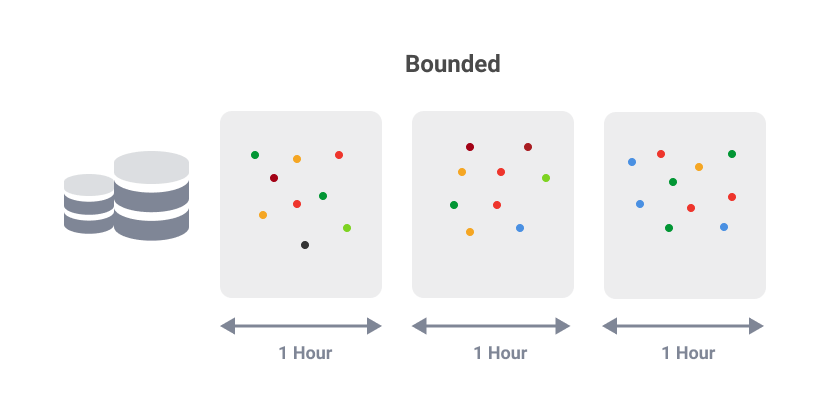
\includegraphics[width=0.7\textwidth]{Images/bounded-data-in-time.png}
                \vspace{1em}
                \caption{Bounded Data in Time}
            \end{figure}
            \begin{figure}[H]
                \centering
                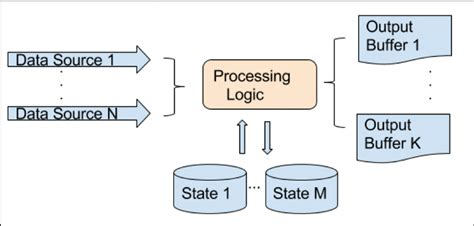
\includegraphics[width=0.7\textwidth]{Images/image (6).png}
                \vspace{1em}
                \caption{processing logic of Incremental Updates}
            \end{figure}
        
        \subsubsection{Tool }
        \begin{figure}[H]
            \centering
            
\includegraphics[width=0.7\textwidth]{Images/arroyo.png}
            \vspace{1em}
            \caption{Arroyo}
        \end{figure}
        We will incorporate \textbf{Arroyo}, a distributed stream processing engine developed in Rust, as part of our technology stack to handle real-time data streams efficiently. Arroyo is designed to support SQL-based queries, making it accessible for processing large volumes of unbounded data streams with ease. Its high scalability ensures that it can handle significant workloads while maintaining \textbf{exactly-once semantics}, which is critical for ensuring data accuracy and consistency. This tool will enable us to implement robust, real-time data processing pipelines, making it an ideal choice for applications requiring low-latency and fault-tolerant stream analytics.
        \begin{figure}[H]
            \centering
            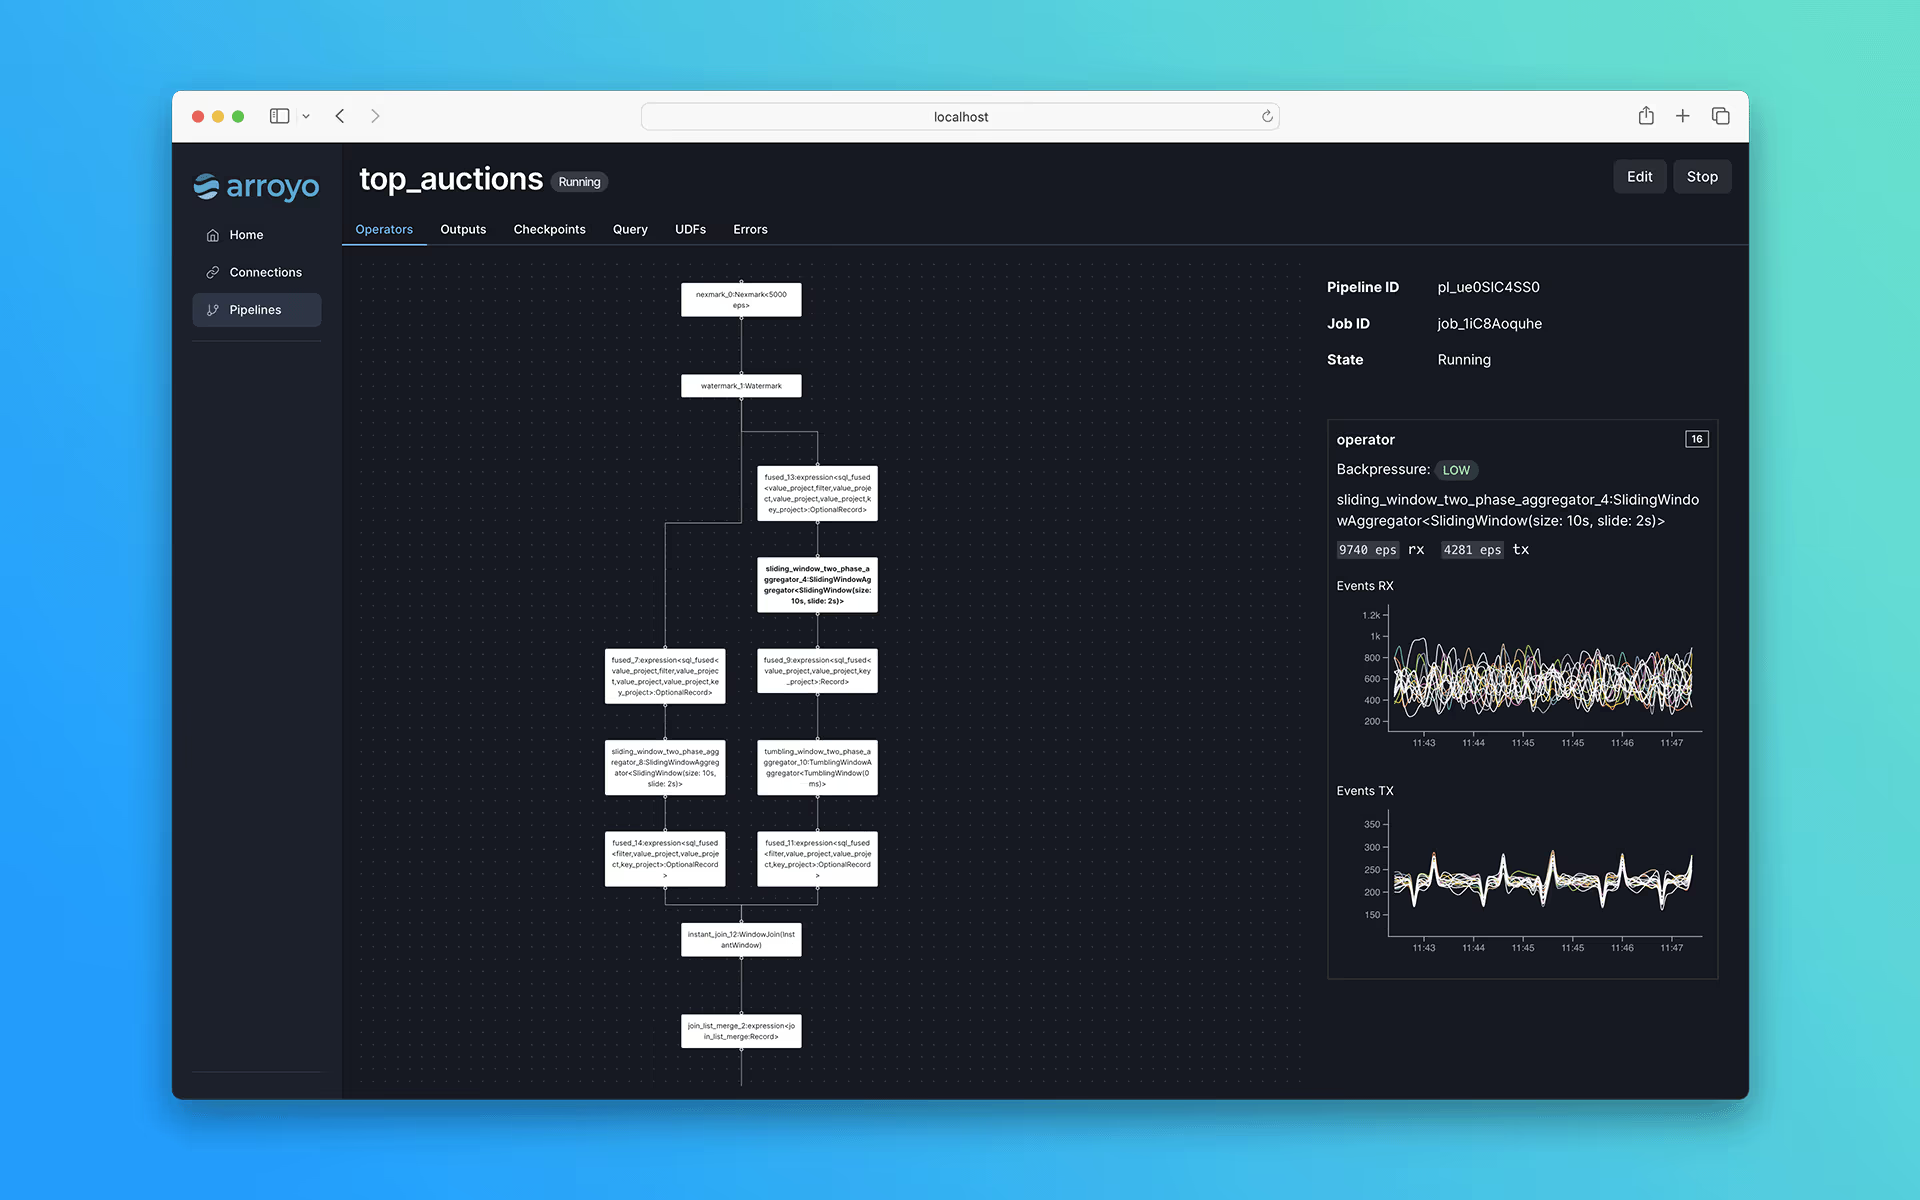
\includegraphics[width=\textwidth]{Images/tool-dash.png}
            \vspace{1em}
            \caption{dashboard}
        \end{figure}

\section{Implementation}
    \subsection{Set Up Infrastructure}
    \subsection{Define Data Pipeline}
    \subsection{Develop Key Tracking Metrics}
    \subsection{Build dashboard}
\section{Conclusion}

\bibliographystyle{plainnat}
\bibliography{refs}

\nocite{*}

\end{document}